\section{Faglig vidensgrundlag}

\subsection{Begrebsdefinitioner} 
De begreber der findes i denne rapport er defineret i tabel \ref{tab:Begrebsdefinitioner}:

% Begrebsdifinitioner
\begin{table}[h]
    \centering
\begin{tabular}{|p{4cm}|p{12cm}|}
\hline
\textbf{Begreb} & \textbf{Definition} \\
\hline
REST API    & REST: \\
            & Repræsentativ tilstandsoverførsel (dansk oversættelse af REST) er en software-arkitektonisk stil, der definerer et sæt begrænsnigner, der skal bruges til at oprettelse af webtjenester\\
            & API: \\
            & API står for Application Programming Interface, og er en softwaregrænseflade, der tillader et stykke software at interagere med andet software \\
\hline
EPG         & EPG er en forkortelse for Electronic Programme Guide. Det er en generelt betegnelse for elektronisk programoversigt over TV-programmer         \\
\hline
GDPR        & Databeskyttelsesforordning, der har til formål at styrke og harmonisere beskyttelsen af personoplysninger i EU \\
\hline
SQL         & Structured Query Language er et programmeringssprog til relationelle databaser\\
\hline
 \end{tabular}
    \caption{Begrebsdefinitioner}
    \label{tab:Begrebsdefinitioner}
\end{table}

\subsection{Metoder og værktøjer}
\begin{longtable}{|p{4cm}|p{12cm}|}
\hline
\textbf{Begreb} & \textbf{Definition} \\
\hline
Brugsmønsterdiagram & Et brugsmønsterdiagram er et diagram der viser hvordan forskellige aktører interagerer med forskellige brugsmønstre \\
\hline
MoSCoW & 
MoSCoW er en prioriterings model der bruges til at sige hvilke ting man: 
\begin{description}[noitemsep]
    \item [Skal] have
    \item [Burde] have 
    \item [Kan] have
    \item [Hvad man ikke] vil have
\end{description}  \\ 
\hline
PostgreSQL          &   PostgreSQL er en open-source objekt-relationel database server.\\
\hline
GitHub              &   GitHub er en web-baseretkollaborations platform henvendt til software udviklere, der gør det muligt at versions-kontrollere projekter.\\ 
\hline
Overleaf            &   Overleaf er en online skriveplatoform for \textbf{LaTeX}, hvor man kan være flere brugere der skriver samtidig. \\
\hline
UML                 &   Unified Modeling Language \\
\hline
IntelliJ            &   Integreret udviklings miljø, som primært bruges af gruppens medlemmer. \\
\hline
ZenHub              &   ZenHub er en platform der gør det lettere at anvende Scrum i praksis.  \\
\hline
Scrum Board         &   \\
\hline
Pair Programming    &   Pair programming er en softwareudvilkingsteknik, hvor to programmører arbejder sammen ved én computer.\\
\hline
Klassediagram       &   Bruges til visuelt at vise hvordan softwaresystemer er opbygget. I diagrammet beskrives systemets klasser, metoder og værdier klassen indeholder, samt klassernes relationer til hinanden.\\
\hline
FURPS+              &   FURPS+ er en model til klassificering af \textit{softwarekvalitetsattributter} % opstil hvad FURPS+ står for, ligesom med Scrum \\
\\
\hline
    \caption{Metoder \& Værktøjer}
    \label{tab:tools}
\end{longtable}

 % Teori --------------------------------------------------------------------------------------------------------
\subsection{Teori}
\subsubsection{Udvikling af brugsmønstermodeller} %-------------------------------
Det første skridt i udviklingen af et brugsmønster er at finde og definere de forskellige aktører der vil interagere med systemet. En aktør kan defineres som alt der kommunikerer med systemet og ikke selv er en del af systemet. Et eksempel på dette kunne være en kunde på en webshop. Disse aktører opstilles i en tabel sammen med de brugsmønstre hver aktør kan tilgå. \\

\noindent
Da kravindsamling er en evolutionær aktivitet, bliver alle aktører ikke nødvendigvis identificeret i første iteration. Det er muligt at identificere primærer aktører i løbet af første iteration, og først senere i forløbet blive i stand til at identificere sekundære aktører, når man får mere viden om systemet. \textit{Primære} aktører interagerer med systemet for at opnå påkrævede systemfunktioner, og ud fra det, få noget ud af at bruge systemet. \textit{Sekundære} aktører støtter systemet så de primærer aktører kan gøre deres arbejde. Når aktørerne er fundet kan brugsmønstrene findes. Et brugsmønster angiver et scenarie en aktør kan interagere med. \\

\noindent
Når både aktører og brugsmønstre er fundet, kan man opstille et brugsmønster-diagram for at give en visuel forståelse for hvilke aktører der kan tilgå hvilke brugsmønstre. Et eksempel på et brugsmønsterdiagram kan ses nedenfor: \\
\begin{figure}[h]
    \centering
    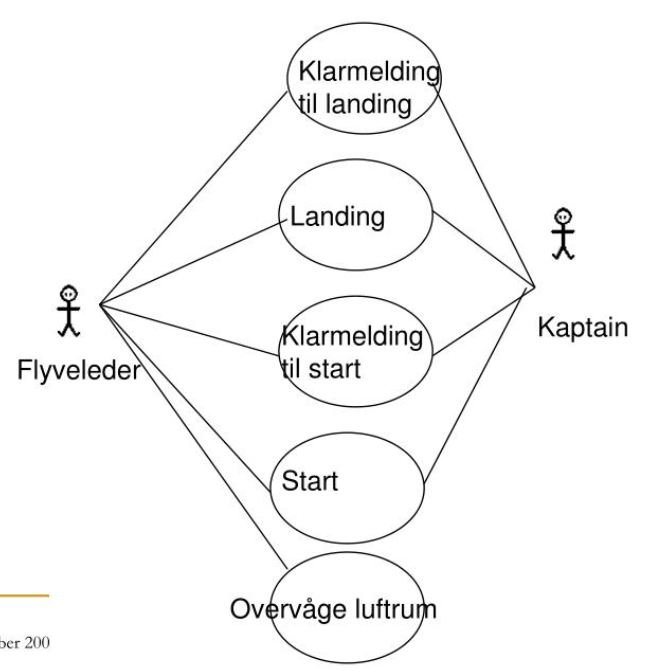
\includegraphics[scale=1]{figures/2. Faglig vidensgrundlag/UseCaseExample.png} \\
    \label{fig:use_case_example}
    \caption{Brugsmønster-diagram eksempel}
\end{figure}
\noindent
Brugsmønstermodellen hjælper udvikleren med at forstå brugeren, så systemet kan konstrueres. Idet der er et samlet billede af hvordan systemet skal se ud, vil udviklingen være mere målfast da kravene og deres forhold til brugeren er klare.


% Fagligt Videngrundlag ----------------------------------------------------------------------------
\subsection{Fagligt Vidensgrundlag}

\subsubsection{JAVA}

\subsubsection{Database}

\subsection{Metoder og værktøjer}

\paragraph{MoSCoW} % ------------------------
MoSCoW er en prioriterings model. Den bruges ofte i software udvikling.\\

\noindent
Modellen i sig selv kan dog bruges, men det anbefaldes at man bruger den sammen med en \textbf{Agile proces}. 
MoSCoW er en vigtig model i software udvikling da, den beskriver hvilken del af softwaren der minimum skal laves før det virker. Der laves en prioritering liste med kunden om hvad de så gerne vil have først. Det bliver så stillet op i en MoSCoW model.

\begin{description}
    \item [Must have] betyder skal have og i software udvikling betyder det, som er minimum der skal være med for at softwaren virker. 
    \item [Should have] betyder det som burde være med det kunden rigtig gerne vil have med.
    \item [Could have] betyder det som kunne være med. Hvis der er tid nok. 
    \item [Won't have (this time)] Det som der slet ikke skal prioriteres nu, men måske en anden gang.
\end{description}